La risposta libera la si calcola azzerando le forze esterne, così facendo
otteniamo l'equazione \ref{eq:free_response}
\begin{equation}
\dot{\bf v}(t)=-\frac{\mu_0}{r^3}{\bf r(t)}, v(0)=v_0 \nonumber
\end{equation}
Per poter simulare l'andamento del satellite in risposta libera, dobbiamo
eliminare tutti i disturbi esterni, come ad esempio il drag, la costante $J_2$
(essa è definita come la seconda armonica zonale e rappresenta l'appiattimento
ai poli del globo terrestre), inoltre bosogna annullare il controllo e spegnere
i propulsori. L'unica forza esterna sarà quella gravitazionale del pianeta
Terra, ma, per rendere la simulazione più ideale, la consideriamo sferica. Per
fare ciò in Matlab impostiamo i seguenti parametri:
\lstinputlisting[language=Matlab]{modelling/orbit_dynamics/code/free_response.m}

Adesso possiamo avviare la simulazione, ottendendo i seguenti plot


\begin{figure}[h]
\begin{center}
  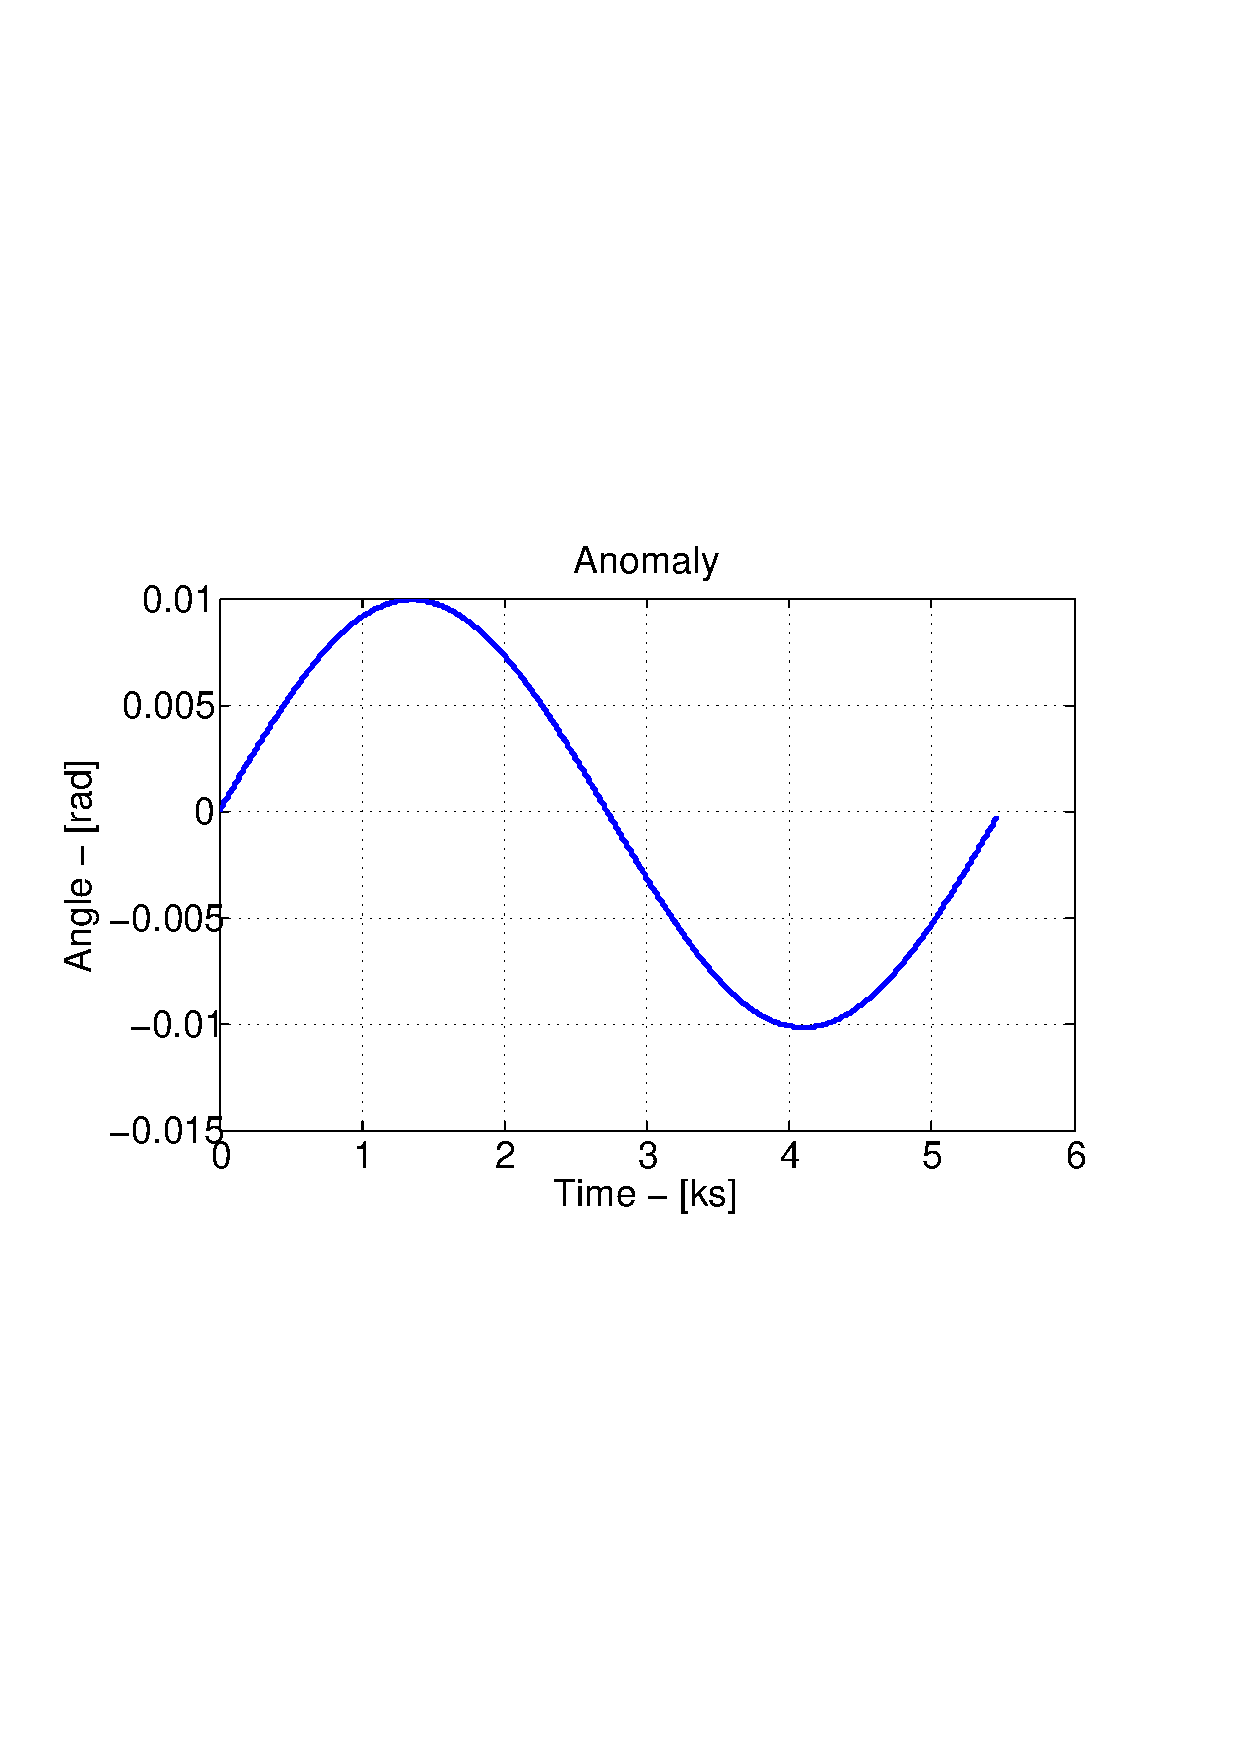
\includegraphics[width=\textwidth,clip=true,trim=2cm
  9cm 2cm 9cm]{modelling/orbit_dynamics/image/anomaly.pdf}
  \caption{Geometria dell'orbita e sistema di riferimento LVLH}
  \label{fig:LVLH}
\end{center}
\end{figure}
